\documentclass[french,10pt,a4paper]{article}	%définition espace pour le document de type article
\usepackage{babel}					%permettre à latex de parler une autre langue que l'anglais (ici le français, mis en option du documentclass)
\usepackage[utf8]{inputenc}			%affichage des caractères accentués
\usepackage[T1]{fontenc}				%affichage des caractères spéciaux
\usepackage{graphicx}				%permet d'insérer des images
\usepackage{subcaption}				%pour créer des sous figures avec légende dans une figure
\usepackage{geometry}				%régler la taille des marges
\setlength{\fboxsep}{8mm}			%définir l'écart de la bordure
\setlength{\fboxrule}{0.3mm} 		%définir l'épaisseur du trait de la bordure
\usepackage{hyperref}				%pour ajouter des hyperliens interactifs
\setcounter{tocdepth}{2}			%profondeur de la table des matières

\usepackage{fancyhdr}				%pour faire une entête
\pagestyle{fancy} 					%Numérotation des pages.
\renewcommand{\headrulewidth}{1pt}

\renewcommand{\abstractname}{Résumé}
\renewcommand{\contentsname}{Table des matières}
\renewcommand{\listfigurename}{Liste des figures}
\fancyhead[L]{\textbf{Rapport Latex Le pendu}}	 		%haut de page gauche
\fancyhead[R]{\textbf{Université Clermont Auvergne}} 	 %haut de page droite
\renewcommand{\footrulewidth}{1pt}
\fancyfoot[L]{Fanny de Weerdt}	 	%pied de page gauche
\fancyfoot[R]{Sasha Baldassin} 	 	%pied de page droit

\renewcommand\headrulewidth{1.5pt}
\makeatletter
\def\headrule{{\if@fancyplain\let\headrulewidth\plainheadrulewidth\fi
\hrule\@height\headrulewidth\@width\headwidth									%commande pour tracer 2 lignes en haut de page
\vskip 2pt		%2pt entre les lignes
\hrule\@height.5pt\@width\headwidth
\vskip-\headrulewidth
\vskip-1.5pt}}
\makeatother

\renewcommand{\footrulewidth}{1pt} %Trace un trait de séparation de largeur d'un point. Mettre 0pt pour supprimer le trait.

\usepackage{listings}				%permet d'afficher un langage de programmation (ici en code python)
\usepackage{color}					%donner une couloration syntaxique aux mots clés du code
\lstdefinestyle{mystyle}{
breakatwhitespace=false} 

\lstset{						%python
basicstyle=\ttfamily,
keywordstyle=\color{blue},		%définition des couleurs pour les lstlisting
commentstyle=\color{green},
numbers=left}

\setlength{\parindent}{0cm}
\setlength{\parskip}{1ex plus 0.5ex minus 0.2ex}
\newcommand{\hsp}{\hspace{20pt}}	%Création de commandes pour gagner du temps dans le code
\newcommand{\HRule}{\rule{\linewidth}{0.5mm}}

\begin{document}
\begin{titlepage}
  \begin{sffamily}
  \begin{center}

    \textsc{\LARGE Rapport Latex}\\[2cm]

    % Titre
    \HRule \\[0.4cm]{\huge \bfseries Le pendu \\[0.4cm]}
    \HRule \\[2cm]
    
    \includegraphics[scale=0.07]{pendu9.png}
    \\[2cm]	%image centrale
    
    \begin{minipage}{0.4\textwidth}
      \begin{flushleft} \large
        \textsc{Binôme 6}\\
        Cohorte : L1 MI-5\\
      \end{flushleft}
    \end{minipage}
    \begin{minipage}{0.4\textwidth}
      \begin{flushright} \large
        \emph{Participant 1 : } \textsc{de Weerdt Fanny}\\
        \emph{Participant 2 : } \textsc{Baldassin Sasha}
      \end{flushright}
    \end{minipage}

    \vfill %termine le paragraphe

    % Bas de page
    {\large 23 Janvier 2023 — 16 avril 2023}

  \end{center}
  \end{sffamily}
\end{titlepage}

\newpage

\begin{abstract}
\noindent	%Enlève l'alinéa
Dans ce projet, nous avons réalisé un pendu : un mot est partiellement affiché, le but : le trouver entièrement en proposant des lettres avec un nombre d'erreurs à ne pas dépasser. \\
Nous avons créé quatre fichiers : \\

\begin{itemize}
\item Un premier : "main.py" qui lance le programme principal avec le menu et contient la partie humain, la partie auto et le turtle. Nous y importons les autres fichiers pour appeler les fonctions permettant de jouer au jeu.\\
\item Un deuxième : "partieauto.py" contenant les fonctions destinées à faire une partie automatique : c'est-à-dire de dérouler une partie de l'ordinateur contre lui-même. L'utilisateur possède plusieurs choix pour le déroulement de cette partie (stratégie de la machine, affichage, ...)\\
\item Un troisième : "interface.py" où se situent toutes les fonctions de l'interface graphique où l'utilisateur a la possibilité de jouer au jeu du pendu hors terminal, que l'on expliquera ici : \ref{tk} \\ %référence à la section où l'on explique l'interface graphique
\item Un dernier : "liste.py" où nous avons créé une grande liste de mots pour le jeu, que l'on expliquera ici : \ref{liste} \\%référence à la section où l'on explique le module faker 
\end{itemize}

Pour finir, nous avons réalisé un menu dans lequel l'utilisateur peut personnaliser sa partie.
\end{abstract}

\newpage
\tableofcontents
\listoffigures
\newpage

\section{Le projet}

\subsection{Organisation}

Nous travaillons ensemble lors des cours de "projet informatique" et à tour de rôle en dehors afin d'éviter les conflits sur git\footnote{Système de gestion de version décentralisé}. Nous nous informons de chaque changement et en discutons ensemble afin d'être en accord sur le rendu. Nous nous partageons le travail au fur et à mesure de l'avancement du projet.

\subsection{Déroulement}

Dans un premier temps, nous avons réalisé toute la partie guidée, partie humain et ordinateur. Puis nous avons réalisé certaines extensions qui nous intéressaient : faire un menu et surtout une interface graphique. Nous nous sommes donc intéressées au développement de cette interface qui nous a pris du temps et avons dû gérer quelques difficultés :
\begin{itemize}
	\item Faire fonctionner python et tkinter ensemble.
	\item Comprendre pourquoi le programme continuait de tourner quand nous effectuions une commande tkinter.
\end{itemize}
Nous avons fait beaucoup de recherches pour comprendre le fonctionnement et surtout gérer les erreurs que nous avions parfois du mal à comprendre.\\
Nous avons réussi à obtenir un résultat qui nous satisfait et avons ainsi pu prendre le temps d'améliorer le visuel et ajouter l'option musique non prévue au départ.\\
Entre temps, nous avons aussi généré une grande liste de mots pour ajouter une plus grande diversité.

\section{Choix d'implémentation des fonctions}


	\subsection{demanderProposition}
	
	
	\begin{lstlisting}[language=Python, frame=single, showspaces=false, showstringspaces=false] 
def demander_proposition(deja_dit,graphisme):	
	lettre = input("Saisir une lettre : ")
	while ( not((lettre>='a' and lettre<='z') or
	(lettre>='A' and lettre<='Z'))) or
		 ((lettre.upper()) in deja_dit) or len(lettre)>1 :  
			if (lettre.upper()) in deja_dit:	 
				print("La lettre a deja ete dite")	 						
			lettre = input("Saisir une lettre : ")
		return lettre.upper() 															
	\end{lstlisting} %frame = single permet d'afficher une bordure
	

	Pour cette fonction, nous avons créé une variable "lettre" où nous demandons à l'utilisateur de saisir une lettre.\\ 
	Une \textit{boucle while} vérifie ces conditions :\\
	
	\begin{itemize}
	\item Une lettre a été saisie (minuscule ou majuscule) et une seule
	\item La lettre n'a pas déjà été dite (vérifié par la recherche dans une liste prise en argument où toutes les propositions ont été ajoutées)
	\end{itemize}
	
	Si ces conditions ne sont pas respectées, on redemande de saisir une lettre. \\
	Pour finir, on retourne la lettre, passée en majuscule.

	
	\subsection{dicoFrequence}
	
	
		\begin{lstlisting}[language=Python, frame=single]
def dico_frequence(nom_fichier) :

	dic_freq_lettre={}	
	f=open(nom_fichier)
	liste=importer_mots (nom_fichier)
	for mot in liste : 								
		indice=0
		for indice in range(len(mot)): 
			if mot[indice] not in dic_freq_lettre : 
				dic_freq_lettre[mot[indice]] = 1 		
			else :
				dic_freq_lettre[mot[indice]]
				 = dic_freq_lettre[mot[indice]] +1 	
	f.close()
	return dic_freq_lettre													
	\end{lstlisting}
	
	On crée un dictionnaire pour stocker chaque lettre avec leur fréquence d'apparition. Les lettres sont les clés et les fréquences sont leur valeur. Après l'ouverture du fichier, une \textit{boucle for} parcourt chaque mot. Dans celle-ci, on initialise une variable "indice" à 0, puis une deuxième \textit{boucle for} permet de parcourir chaque lettre du mot grâce à la variable "indice" qui s'incrémente de 1 jusqu'à la longueur du mot . \\
	On vérifie si la lettre est présente dans le dictionnaire, si c'est le cas on rajoute 1 à la valeur, sinon on crée la clé initialisée à la valeur à 1. \\
	Une fois toutes les lettres parcourues, la première boucle permet de changer de mot et le processus reprend. \\
	On renvoie le dictionnaire.
	
	
	\subsection{fabriqueListeFrequence}
	
	\begin{lstlisting}[language=Python, frame=single]
def fabrique_liste_freq(nom_fichier) :

	liste_freq=[]
	dic=dico_frequence(nom_fichier)								 
	while len(dic)>0 :
		lettre = lettre_la_plus_frequente(dic)					
		liste_freq.append(lettre)
		del dic[lettre]											
	return liste_freq
	\end{lstlisting}
	
	Cette fonction permet de renvoyer la liste des lettres contenues dans un fichier de la plus fréquente à la moins fréquente. Pour cela on fait appel à la fonction "dicoFrequence" pour connaître la fréquence de chaque lettre puis à la fonction "lettreLaPlusFrequente" afin de les classer par ordre décroissant dans la liste créée. On supprime la dernière lettre parcourue pour passer à la suivante.
	
\section{Extensions}


	\subsection{Menu}
	
	
	Pour le menu, nous avons fait un programme basé sur des choix par oui/non ou des numéros. \\
	Nous affichons dans le terminal chaque choix que l'utilisateur peut faire pour personnaliser sa partie, l'utilisateur entre le numéro de son choix ce qui engendre l'affichage de nouveaux choix selon le précédent jusqu'au lancement de la partie. \\
	Ce menu fonctionne grâce à une succession de conditions (dans des \textit{if}). Les blocs d'instructions fonctionnent grâce à des variables représentant chaque choix de l'utilisateur. Arrivé à terme, un appel de fonction est effectué respectant chaque choix de l'utilisateur et lance la partie correspondante.
	
	
	\subsection{Ascii Art}
	
	
	\begin{minipage}{.6\textwidth}
	Afin de rendre le jeu plus traditionnel, nous avons décidé de "dessiner" un pendu dans le terminal.\\	
	Nous avons créé une liste de 10 éléments. A chaque erreur nous appelons l'indice de la liste correspondant. Le premier élément est vide car au lancement de la partie il n'y a pas d'erreur. Au fur et à mesure nous ajoutons un morceau du pendu dans la liste. 	
	\end{minipage}		
	\hfill	
	\begin{minipage}{.27\textwidth}		%minipage pour afficher l'image et le texte à côté
	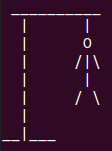
\includegraphics[width=\textwidth]{penduascii.png}	%affichage de l'image
	\captionof{figure}{pendu ASCII}	
	\end{minipage}
	
	\subsection{Interface graphique}
	
	
	\subsubsection{Modules à installer}
	
	Commandes à utiliser sous Ubuntu/Debian :
	\begin{itemize}
	\item Tkinter : sudo apt-get install python3-tk	%module interface tkinter
	\item Pygame (musique) : pip install pygame		%module pour la musique
	\item Pillow (image) : python3 -m pip install --upgrade Pillow %module pour afficher les images
	\item Turtle : python3 -m pip install --user PythonTurtle %module interface turtle
	\end{itemize}
	
	
		\subsubsection{Tkinter}
		
		
		\label{tk} Quand l'utilisateur choisit l'option graphique, cela lance l'interface tkinter en plein écran qui lui propose diverses fonctionnalités : %référence pour cliquer dessus quand nous sommes sur le résumé
		
		\begin{itemize}
		\item Lancer une partie
		\item Lire les règles du jeu
		\item Option pour mettre/enlever la musique
		\item Quitter le jeu
		\end{itemize}
		
		Ces quatre possibilités fonctionnent grâce à des boutons appelant des fonctions. \\
		Quand le jeu est lancé, 26 boutons, correspondant aux lettres, apparaissent pour trouver un mot mystère qui est sous forme de tirets. \\
		Quand le joueur clique sur un bouton, il se grise et devient alors inutilisable. Si la lettre ne fait pas partie du mot, il a une erreur de plus, si elle en fait partie, elle remplace le tiret correspondant.\\
		Nous affichons la mise en scène du pendu avec des photos de playmobils à chaque nouvelle erreur. \\
		Quand la partie est finie, le joueur peut retourner au menu et le processus recommence.\\
		De plus, une musique, composée par Sasha, se lance à l'ouverture de l'interface. Le joueur peut décider de couper ou de remettre le son. \\
		Nous avons mis toutes les fonctions dans le fichier "interface".
		
		\begin{figure}[!ht]
			\begin{subfigure}{0.5\textwidth}
    				\centering
    				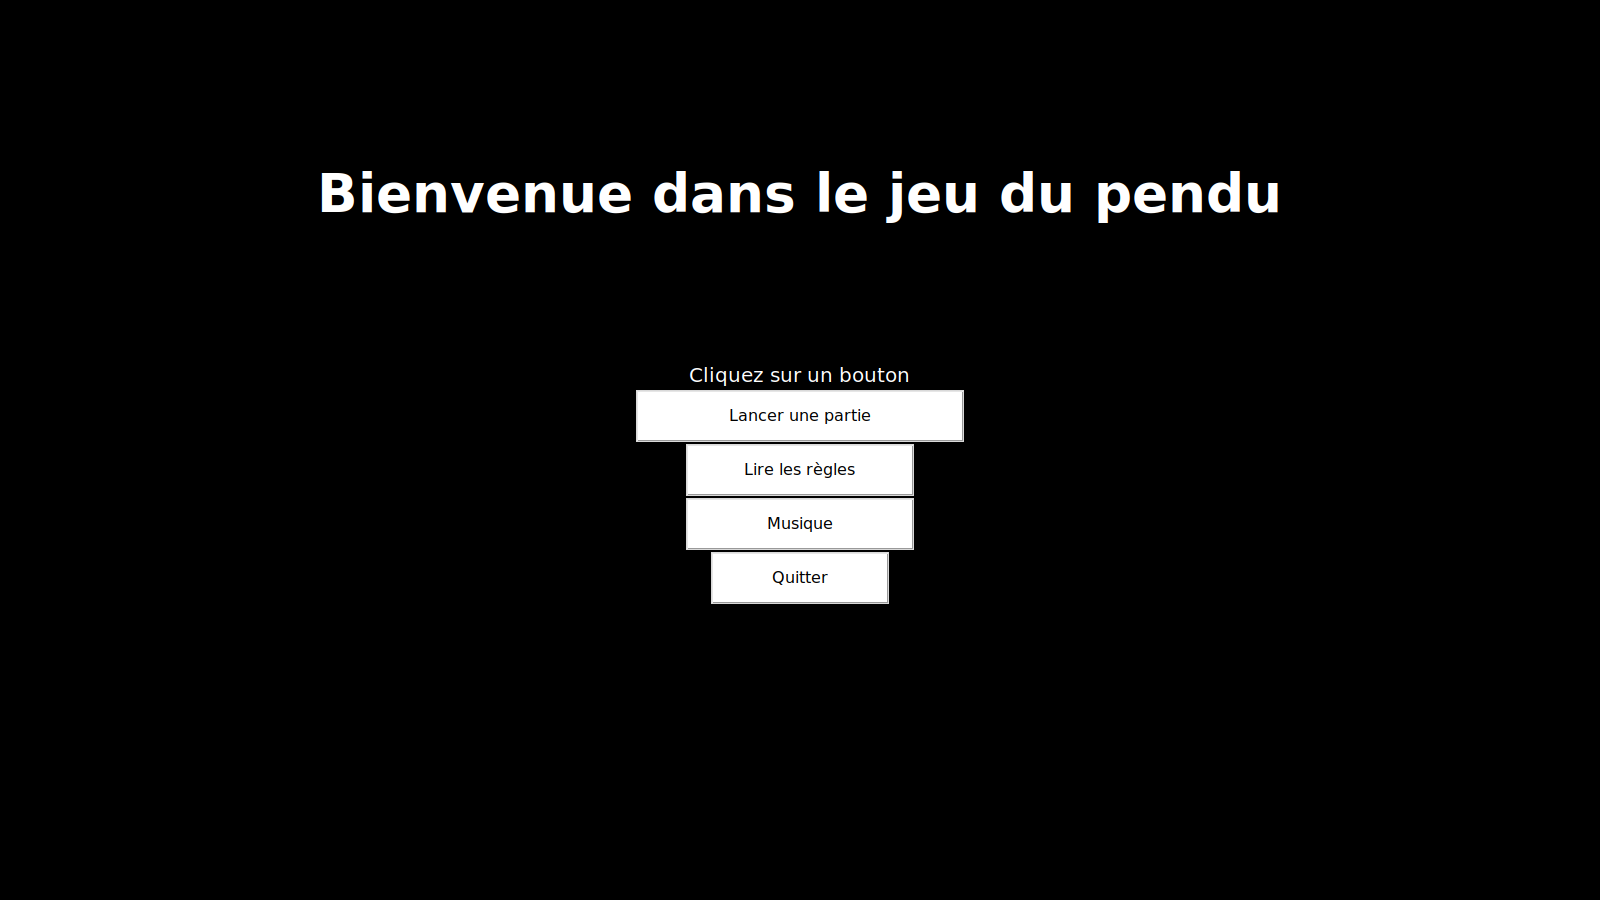
\includegraphics[scale=0.1]{accueil.png}
   		 			\caption{Le menu}
   		 			\centering
			\end{subfigure}
			\begin{subfigure}{0.5\textwidth}
   			 		\centering
    				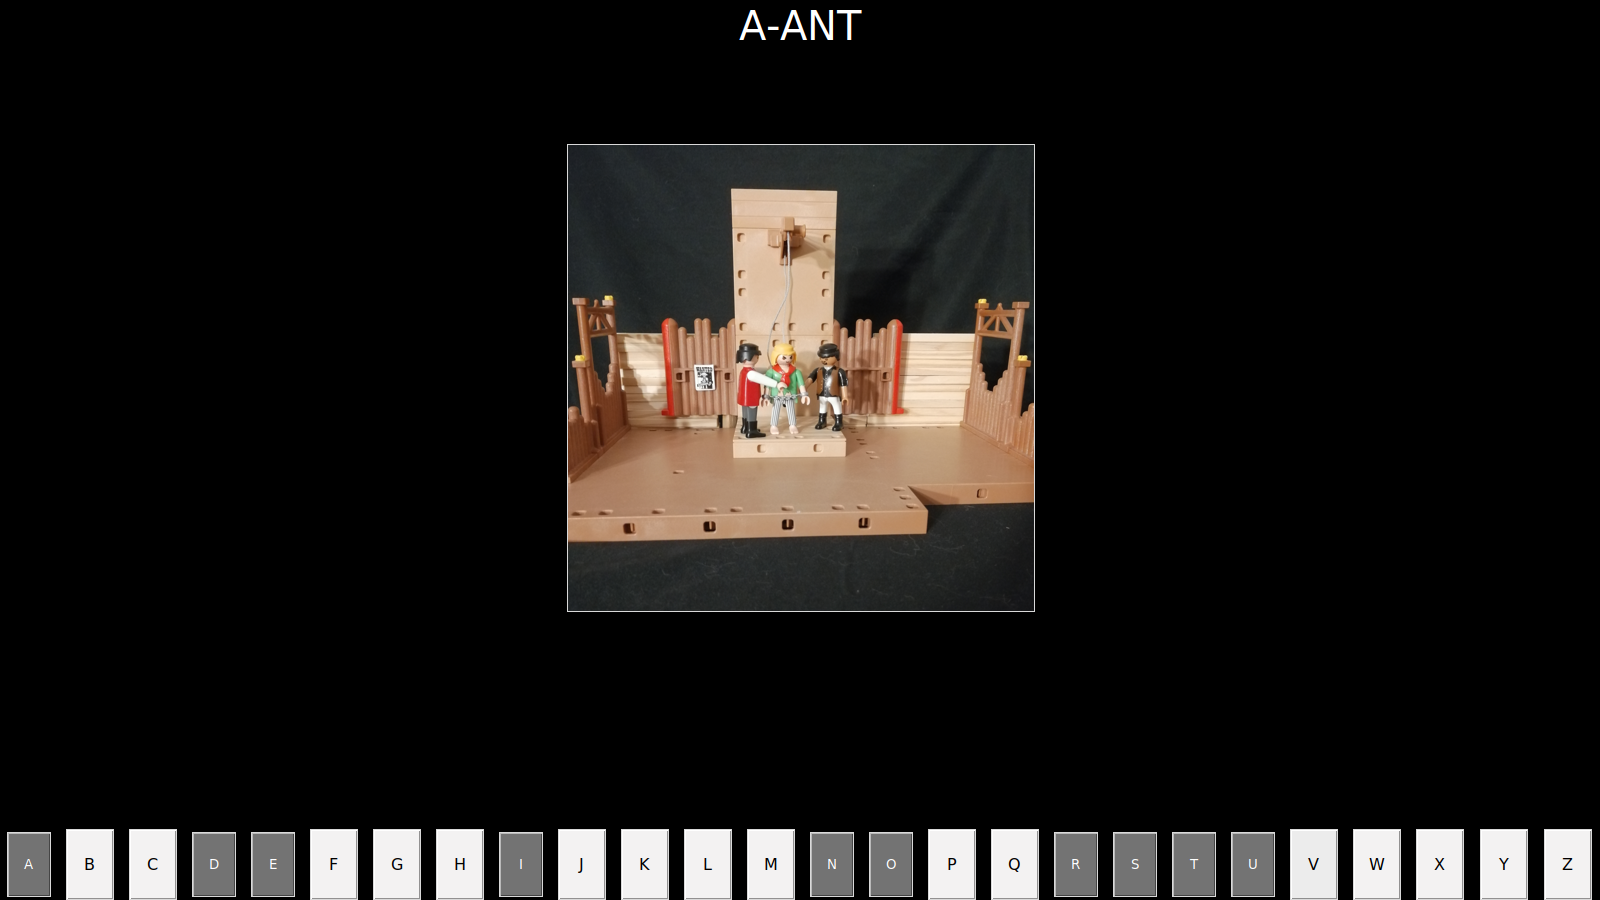
\includegraphics[scale=0.1]{jeu.png}
    				\caption{Le jeu}
    				\centering
			\end{subfigure}
    			\caption{Interface tkinter}
		\end{figure}
		
		\subsubsection{Turtle}
		
		
		Nous avons choisi d'utiliser turtle pour dessiner un pendu bâton en utilisant les commandes basiques de ce module. \\
		L'utilisateur peut activer cette option uniquement s'il fait le choix "partie humain". Une autre fenêtre s'ouvre en se positionnant à droite lorsque l'utilisateur commet sa première erreur.\\
		Nous utilisons des commandes qui créent une partie supplémentaire du pendu à chaque nouvelle erreur.\\
	 Le jeu se termine lorsque le joueur gagne ou qu'il perd et que le pendu est entièrement affiché. La fenêtre se ferme à la fin de la partie.
		
		
	\subsection{Génération liste de mots}
	
	
	\label{liste} Dans le fichier "liste", nous avons utilisé le module Faker pour générer une liste de mots. \\
	Dans celui-ci, nous ouvrons notre fichier de mots et une \textit{boucle for} effectue 10000 itérations pour créer 10000 mots et les écrit un par ligne. \\
	
	\begin{lstlisting}[language=Python, frame= single]
from faker import Faker
fake = Faker('fr_FR')
with open('fichiermots.txt','w') as f :
	for i in range(10000):
		mot = fake.word()
		f.write(mot + '\n')
	\end{lstlisting}
	
		Nous avons choisi la langue française, et pour éviter les problèmes de caractères non ASCII, nous avons modifié la fonction "importer\_ mots" \\
	En effet, nous avons rajouté une boucle for et créé une variable initialisée à \textit{True} où l'on vérifie que tous les caractères du mot sont des lettres appartenant au code ASCII\footnote{Norme informatique de codage de caractères}. La variable devient alors \textit{False} si un caractère non ASCII est trouvé (caractères accentués, cédille, etc).\\
		
	\begin{lstlisting}[language=Python, frame= single]
def importer_mots (nom_fichier) :
    f=open(nom_fichier)
    l1=[]
    for ligne in f :
        a=True
        ligne = ligne.strip() 			
        for j in range(len(ligne)) :
        	if not ((ligne[j]>='A' and ligne[j]<='Z')
        	 or (ligne[j]>='a' and ligne[j]<='z')) :
        	     a=False
        if a :
               ligne = ligne.upper() 			
               if len(ligne)>=3 :            
                    l1.append(ligne) 				
    f.close()
    return l1
	\end{lstlisting}
	
\newpage
\section{Programme principal}


	\subsection{Contenu}
	
	
	Le programme principal est présenté sous forme de menu. Il contient chaque option du jeu :
	
	\begin{itemize}
	\item Choix de l'interface graphique
	\item Menu du jeu : jouer, lire les règles, quitter
	\item Mode de jeu (humain ou ordinateur)
		\begin{itemize}		
		\item[-] Si partie humain :
			\subitem . Choix de l'affichage turtle ou non
		\item[-] Si partie auto :		
			\subitem . Choix d'un affichage ou non
			\subitem . Si oui avec des pauses ou non
			\subitem . Stratégie de l'ordinateur
		\end{itemize}	
	\item Quitter le jeu	
	\end{itemize}
	
	Le programme principal commande les appels de fonction et l'interaction avec l'utilisateur.
		
	\subsection{Fonctionnement}
	
	
	Dans le programme principal, nous demandons d'abord si l'utilisateur souhaite une interface graphique ou non. Si c'est le cas, la fenêtre tkinter est créée et lance une fonction qui permet de boucler le programme et de lancer la partie. Le programme s'arrête et la fenêtre se ferme lorsque l'utilisateur clique sur quitter.\\ 
	Sinon le reste du menu s'affiche selon les choix de l'utilisateur dont l'option pour afficher un pendu dans une autre fenêtre avec turtle. Ce programme est dans une \textit{boucle while} où se situent tous les choix possibles pour lancer une partie et la boucle s'arrête lorsque l'utilisateur choisit de quitter (numéro 3 du menu).\\
Le programme principal se situe dans le fichier "main.py". En effet c'est celui qu'il faut lancer, il relie les 3 fichiers et gère tous les appels de fonctions selon les choix de l'utilisateur.

\section{Séparation en plusieurs fichiers}

	Nous avons séparé le code en plusieurs fichiers pour le rendre plus aéré et plus lisible.\\
	En effet, toutes les fonctions prenaient beaucoup de lignes et nous avions du mal à nous repérer.\\
	Nous avons donc découpé en quatre fichiers : programme principal, fonctions de la partie automatique, tkinter et le fichier de mots.\\
	Nous avons laissé la fonction "partie auto" dans le fichier principal car il représente la partie guidée, nous avons juste mis les fonctions de cette partie à part.


\section{Perspectives}
	
	Avec plus de temps, nous aurions aimé réaliser d'autres extensions, notamment travailler une partie statistiques qui aurait été très intéressante autant d'un point de vue mathématiques que d'un point de vue algorithmique.\\
	Nous aurions aussi pu créer différents niveaux de difficultés pour rendre le jeu moins lassant sur la durée.\\
	Nous aurions également mieux organisé la séparation du code en différents fichiers afin que ce soit plus clair et facile d'utilisation.	

\section{Le gitlab}
Vous trouverez \href{https://gitlab.com/de-weerdt-baldassin/le-pendu}{\textbf{ici}} le lien pour le gitlab. %lien cliquable

\section{Bibliographie}

\begin{itemize}
\item \href{https://python.doctor/page-tkinter-interface-graphique-python-tutoriel}{python.doctor} 
\item \href{https://htmlcolorcodes.com/fr/}{htmlcolorcodes.com} %lien des références consultées
\item \href{https://stackoverflow.com/questions/42828416/print-output-in-gui-interface-tkinter-python}{stackoverflow.com}
\end{itemize}

\end{document}